\documentclass{beamer}

\usepackage[T1]{fontenc}
\usepackage[ngerman]{babel}
\usepackage[utf8]{inputenc}
% diese drei Pakete
% in dieser
% Reihenfolge
\usepackage{tabularx}
\beamertemplatenavigationsymbolsempty

\author{Hier eure Namen eintragen, Philipp}
\title{Clickbait Detection}
\begin{document}
%\item[\textbf{+}] #1
\newcommand{\pro}[1]{\item[\colorbox{green}{\textcolor{white}{\makebox(5.5,7){\textbf{+}}}}] #1}
\newcommand{\con}[1]{\item[\colorbox{red}{\textcolor{white}{\makebox(5.5,7){\textbf{--}}}}] #1}
\begin{frame}
\titlepage
\end{frame}

\section{Albacore Clickbait Detection}
\begin{frame}
\frametitle{Albacore Clickbait Detection}
    \begin{definition}
    %Headers of news articles that have misleading titles and exaggerate the content of the news
	%articles to create misleading expectations for users are called clickbaits   
	Eine Vorschau eines Nachrichtenartikels, die einen irreführenden Titel oder übertriebenen Inhalt enthält, um falsche Erwartungen 
	beim Benutzer zu erzeugen, heißt Clickbait.
	\end{definition}
\end{frame}
\begin{frame}
    \frametitle{Zielsetzung}
	\begin{itemize}    
	\item Regressor Modell vorstellen, das die Wahrscheinlichkeit angibt, mit der ein Post Clickbait ist.
	\item Mean Sqaured Error auf Datensatz der Clickbait Challenge minimieren.
	\end{itemize}
\end{frame}
\begin{frame}
    \frametitle{Beschreibung}
    \begin{figure}
  	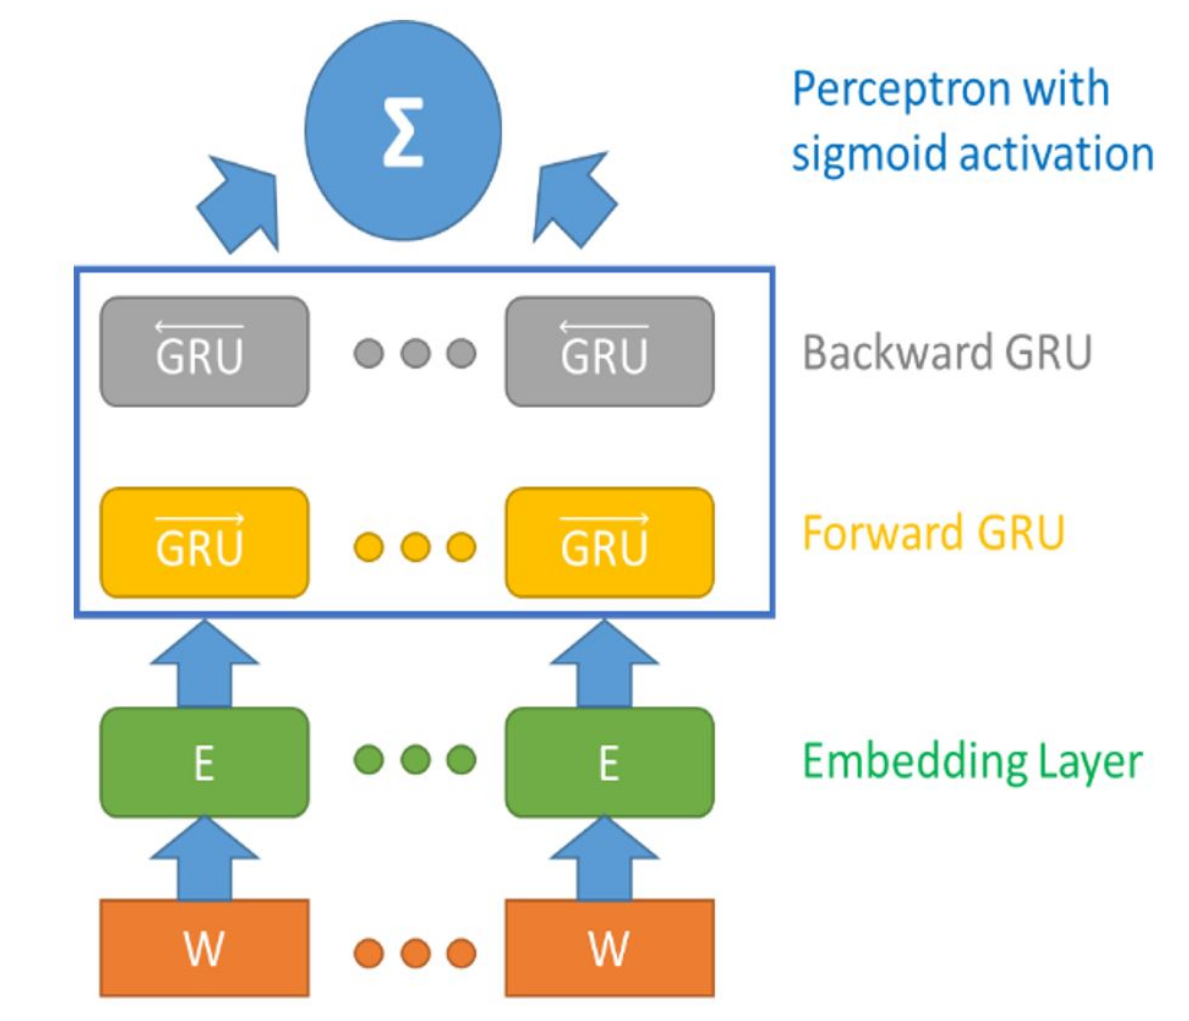
\includegraphics[width=0.8\linewidth]{albacore.png}
\end{figure}
\end{frame}
\begin{frame}
    \frametitle{Evaluierung}
    \center
    \begin{tabular}{c|c}
    Metrik & Ergebnis \\ \hline 
    Mean Squared Error & 0.0315 \\
	Median Absolute Error & 0.122 \\
	F1 Score & 0.670 \\
	Precision & 0.732 \\
	Recall & 0.619 \\
	Accuracy & 0.855 \\
	R2 Score & 0.571 \\
	Runtime & 00:01:10 \\
    \end{tabular}
	
	\begin{itemize}
	\item Clickbait Challenge 2017 gewonnen
	\end{itemize}
\end{frame}
\begin{frame}
    \frametitle{Kritik}
    \begin{itemize}
	\pro{Kleiner Mean Squared Error}
	\pro{Einfaches Modell}
	\con{Nur \texttt{postText} benutzt}
	\end{itemize}
\end{frame}

\section{Zingel Clickbait Detector}
\begin{frame}
\frametitle{Zingel Clickbait Detection}
    \begin{definition}
    %Headers of news articles that have misleading titles and exaggerate the content of the news
	%articles to create misleading expectations for users are called clickbaits   
	Clickbait bezeichnet etwas (wie z.B. eine Überschrift), das so entworfen wurde, dass Leser auf einen Hyperlink klicken wollen,
	insbesondere, wenn der Link zu Inhalten dubiosen Interesses oder Wertes führt.
	\end{definition}
\end{frame}
\begin{frame}
    \frametitle{Zielsetzung}
	\begin{itemize}    
	\item Automatisierten Ansatz entwickeln, um Clickbait aus Twitter Stream zu filtern.
	\item Mean Sqaured Error auf Datensatz der Clickbait Challenge minimieren.
	\end{itemize}
\end{frame}
\begin{frame}
    \frametitle{Beschreibung}
    \begin{figure}
  	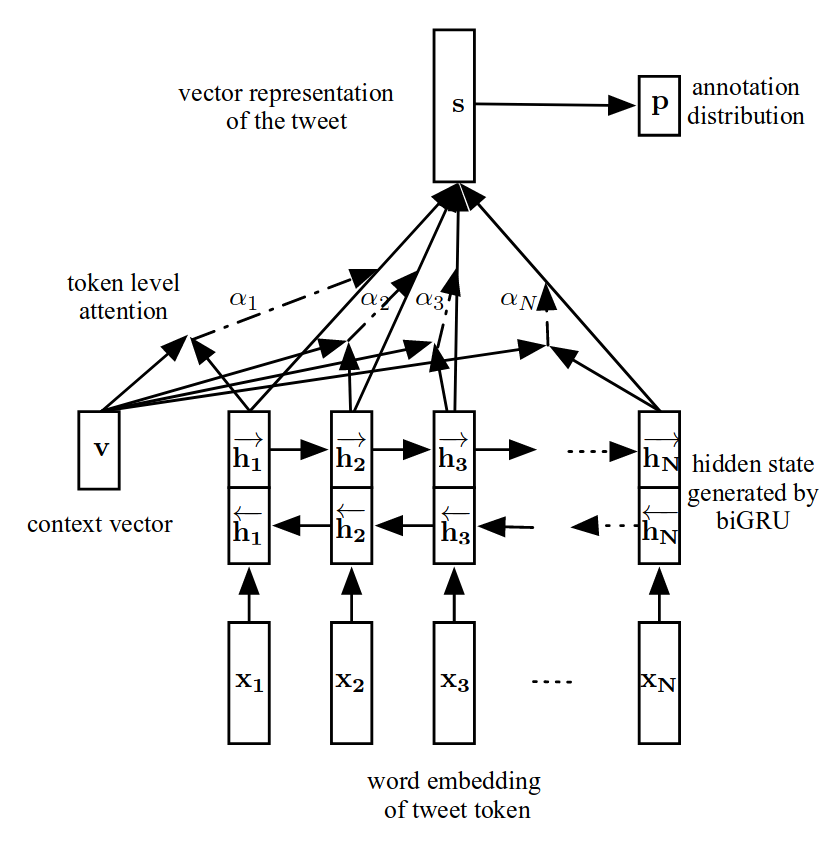
\includegraphics[width=0.7\linewidth]{zingel.png}
\end{figure}
\end{frame}
\begin{frame}
    \frametitle{Evaluierung}
    \center
    \begin{tabular}{c|c}
    Metrik & Ergebnis \\ \hline 
    Mean Squared Error & 0.0333 \\
	F1 Score & 0.683 \\
	Accuracy & 0.856 \\
	Runtime & 00:03:27 \\
    \end{tabular}
	
	\begin{itemize}
	\item Zweiter Platz bei Clickbait Challenge 2017
	\end{itemize}
\end{frame}
\begin{frame}
    \frametitle{Kritik}
    \begin{itemize}
	\pro{Kleiner Mean Squared Error}
	\pro{Einfaches Modell}
	\con{Komplizierter als Albacore, trotzdem schlechter}
	\con{Nur \texttt{postText} benutzt}
	\end{itemize}
\end{frame}

\end{document}
